%roughly 2-3 pages
%\begin{itemize}
%\item any details about experiments (dataset sizes, parameter selection, etc)
%\item results
%\item analysis (discussion of results/visualizations/findings/etc)
%\end{itemize}

The experiments have been run on a dataset consisting of $9.728$ labeled documents. Different parameters may influence the accuracy of the classifier.These are $\alpha$, the Dirichlet parameter for $\theta$, $\beta$, the Dirichlet parameter for $\varphi$, the number of topics to be extracted from the dataset and the number of iterations for Gibbs sampling. 
For validation, k-fold cross-validation has been used with $k=5$ (as described in section \ref{sec:fold}), to ensure an unbiased test. Table \ref{table:genre_sizes} shows the number of documents in the dataset for each genre.

\begin{table}[htp!]
\begin{center}
\scalebox{0.7}{
\begin{tabular}{|c|c|c|c|c|c|c|c|c|c|c|c|} 
\hline
Genre & Reggae & Latin & Holiday & Stage \& Screen & Electronic & Children's & Country & Jazz & Vocal & Easy Listening & New age \\
\hline
\# Documents & 65 & 67 & 11& 121 & 330 & 60 & 679 & 138 & 259 & 28 & 21 \\
\hline
\hline
Genre & R\&B & Avant-Garde & Pop/Rock & Folk & Rap & International & Blues & Comedy/Spoken & Religious & Classical & Total\\
\hline
\# Documents& 785 & 6 & 5470 & 129 & 720 & 186 & 101 & 35 & 470 & 47 & 9728\\
\hline
\end{tabular}}
\caption{Number of documents per genre}
\label{table:genre_sizes}
\end{center}
\end{table}


\subsection{Cross-validation}\label{sec:fold}
Cross-validation is a validation technique to asses how the results of the models will generalize. In this research a stratified 5-fold cross-validation is implemented. In 5-fold cross-validation, the dataset is split into 5 equal size subsets and the algorithm is performed 5 times (or folds) in which one of the 5 subsets is used as validation data. Each experiment is thus run 5 times where the training set entails 80\% of the total data set and the validation set entails 20\% of the total dataset. Due to the variation in population for each genre in the dataset, a stratified sampling of training and validation set for the subsets is used. This sampling technique preserves the percentage of samples for each class in all subsets.


\begin{figure}[htp!]
\begin{mdframed}
        \centering
        \begin{subfigure}[b]{0.3\textwidth}
                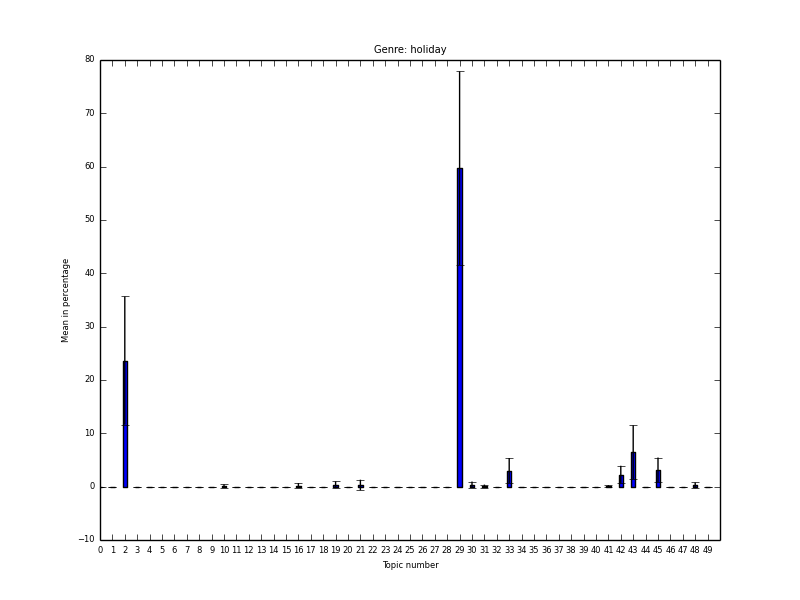
\includegraphics[width=\textwidth]{bar_charts/holiday.png}
                \caption{Genre Holiday}
                \label{fig:topicdist_holiday}
        \end{subfigure}%
        ~ %add desired spacing between images, e. g. ~, \quad, \qquad, \hfill etc.
          %(or a blank line to force the subfigure onto a new line)
        \begin{subfigure}[b]{0.3\textwidth}
                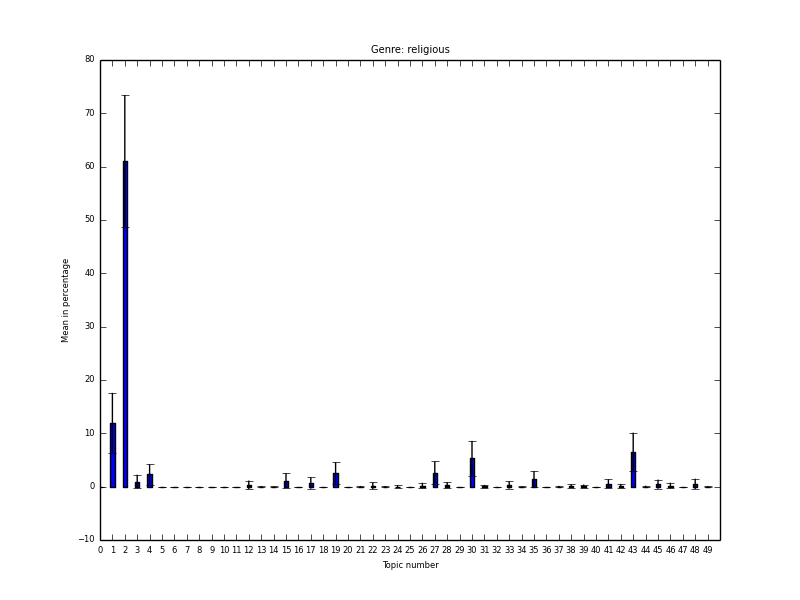
\includegraphics[width=\textwidth]{bar_charts/religious.png}
                \caption{Genre Religious}
                \label{fig:topicdist_religious}
        \end{subfigure}
        ~ %add desired spacing between images, e. g. ~, \quad, \qquad, \hfill etc.
          %(or a blank line to force the subfigure onto a new line)
        \begin{subfigure}[b]{0.3\textwidth}
                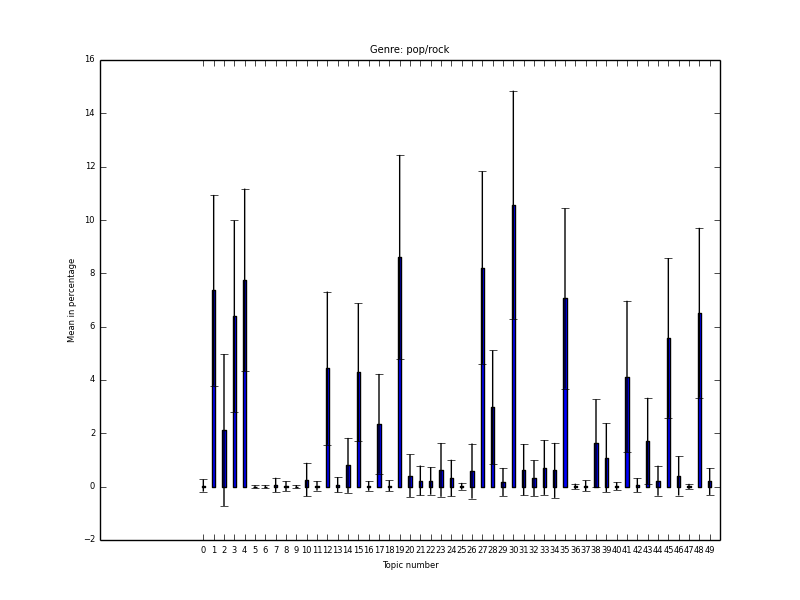
\includegraphics[width=\textwidth]{bar_charts/pop-rock.png}
                \caption{Genre Pop/Rock}
                \label{fig:topicdist_poprock}
        \end{subfigure}
        \begin{subfigure}[b]{0.3\textwidth}
                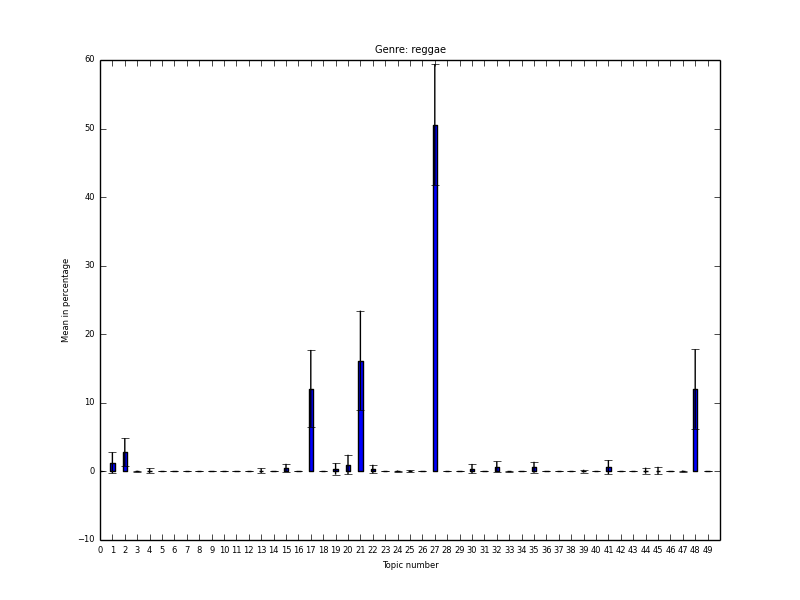
\includegraphics[width=\textwidth]{bar_charts/reggae.png}
                \caption{Genre Reggae}
                \label{fig:topicdist_reggae}
        \end{subfigure}%
        ~ %add desired spacing between images, e. g. ~, \quad, \qquad, \hfill etc.
          %(or a blank line to force the subfigure onto a new line)
        \begin{subfigure}[b]{0.3\textwidth}
                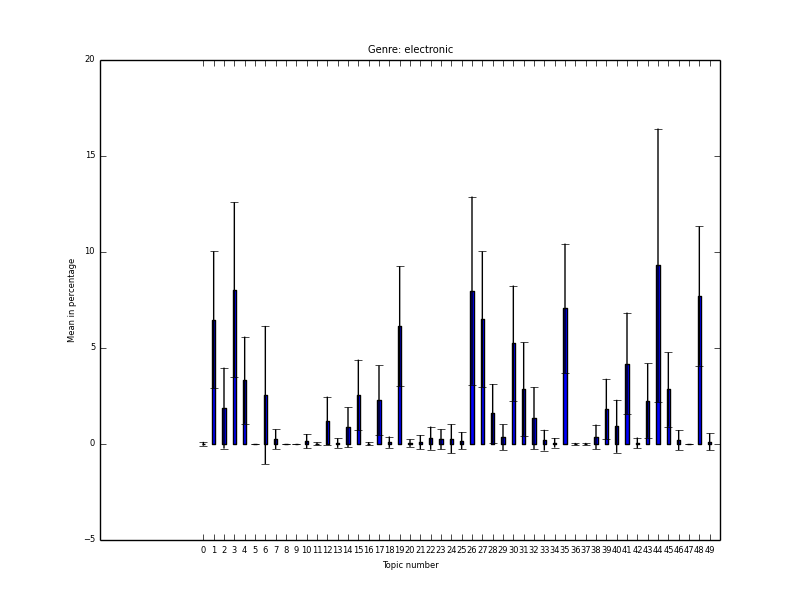
\includegraphics[width=\textwidth]{bar_charts/electronic.png}
                \caption{Genre Electronic}
                \label{fig:topicdist_electronic}
        \end{subfigure}
        ~ %add desired spacing between images, e. g. ~, \quad, \qquad, \hfill etc.
          %(or a blank line to force the subfigure onto a new line)
        \begin{subfigure}[b]{0.3\textwidth}
                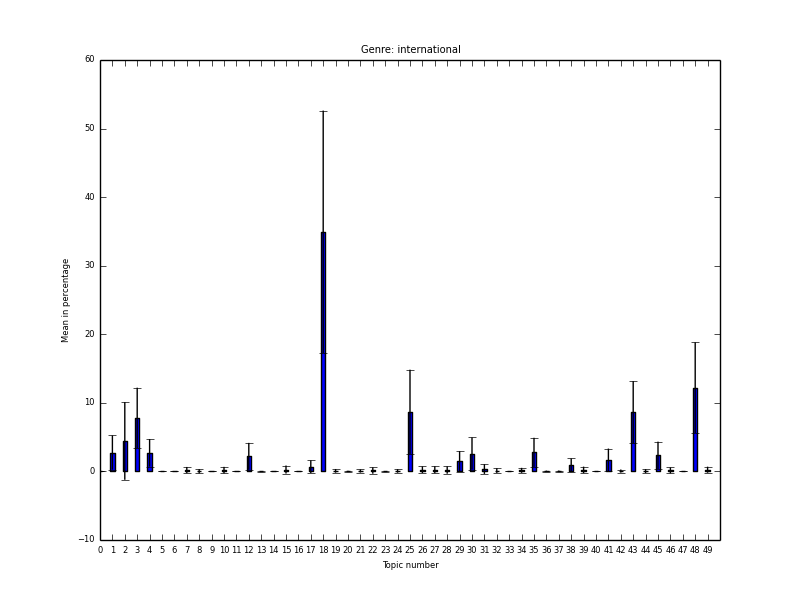
\includegraphics[width=\textwidth]{bar_charts/international.png}
                \caption{Genre International}
                \label{fig:topicdist_international}
        \end{subfigure}
        \caption{Topic distibution for different genres}\label{fig:topicdist}
\end{mdframed}
\end{figure}



\subsection{Results}
Figure \ref{fig:topicdist} presents genre profiles for different genres. Each profile is created by summing topic counts for every document in the genre, and averaging these. These profiles are strongly dominated by one or two topics for certain genres, like \textit{Holiday}, \textit{Religious} and \textit{Reggae}, but more evenly distributed for others, like \textit{Electronic} or \textit{Pop/Rock}. This is not surprising, as \textit{Holiday} and \textit{Religious} are genres named after the themes of their songs, and not their musical structure. Moreover, \textit{Pop/Rock} contains music styles ranging from pop music to brutal death metal, resulting in a genre profile that covers a wide range of topics. Results of the classification using the extended LDA and original LDA model can be found in table \ref{tab:poprock100}. Results show that by applying more topics for the model, the performance of the classifier will increase. The classifiers have scores of around 50\%. However, at close inspection of the classifications, it showed that the classifiers almost always predicted the genre Pop/Rock. Since more than half of the dataset consists of data labeled with \textit{Pop/Rock}, it is unsurprising that the classifier didn't work too well. 
\begin{table}[h]
\begin{tabular}{|l|r|r|r|}

\hline
\textbf{Type of LDA} &  \textbf{Average Precision} & \textbf{Average Recall} & \textbf{Average F1} \\
\hline
Extended &0.50310266811037774 & 0.59352517985611508 & 0.48576895832520584 \\
Original & 0.31608099763575387 & 0.56166495375128467 & 0.40451708979848938 \\
\hline
\end{tabular}
\caption{Classification including pop/rock genre, Topics = 100, alpha=0.1, beta=0.1}
\end{table}

Consequently, the same experiment was re-run, leaving out the data labeled \textit{Pop/Rock}. \footnote{This only concerns the experiment with 50 topics due to time constraints.} As a result of the removal of Pop/Rock, the dataset consisted of $4.258$ documents. The results of running extended and original LDA without \textit{Pop/Rock} documents can be found in table \ref{tab:difflda}. These results show that extended LDA outperforms original LDA. Moreover, the most distinctive topics were \textit{R\&B} and \textit{Rap}. Higher results were expected for \textit{Holiday} and \textit{Religious} and \textit{Reggae}, due to their distinctive genre profiles. However, the size of \textit{Holiday} and \textit{Reggae} was relatively small (11 and 65 documents). However, \textit{Religious} is a rather large part of the dataset. Further analysis showed that most documents belonging to the genre \textit{Religious} were predicted to be \textit{Country}, which is a larger subset of the dataset. Since \textit{Country} is a genre associated with the conservative American South, it might share a lot of themes with \textit{Religious} (allusions to God and Heaven, for example). 
\begin{table}[h!]
\centering
\begin{subtable}[b]{0.8\textwidth}
\begin{tabular}{| r | r | r | r | r | r | r |}
\hline
\textbf{Folds} &  \textbf{1} & \textbf{2} & \textbf{3} & \textbf{4} & \textbf{5} & \textbf{Average}\\
\hline
avant-garde & 0 & 0 & 0 & 0 & 0 & 0\\
blues & 0 & 0.0011 & 0.0023 & 0 & 0 & 0.0007\\
children's & 0 & 0 & 0.0012 & 0.0023 & 0 & 0.0007\\
classical & 0 & 0  & 0.0023 & 0 & 0 & 0.0005\\
comedy/spoken & 0 & 0 & 0.0023 & 0 & 0 & 0.0005 \\
country & 0 & 0.1357 & 0.0982 & 0.0983 & 0.0962 & 0.0857 \\
easy listening & 0 & 0 & 0 & 0 & 0 & 0 \\
electronic & 0 & 0.0093 & 0.0548 & 0.0681 & 0.0047 & 0.0274\\
folk & 0 & 0 & 0.0023 & 0 & 0.0047 & 0.0014\\
holiday & 0 & 0 & 0 & 0 & 0 & 0 \\
international & 0 & 0.0070 & 0.0117 & 0.0232 & 0.0163 & 0.0116\\
jazz & 0 & 0 & 0.0023 & 0 & 0.0209 & 0.0046 \\
latin & 0 & 0 & 0.0023 & 0.0023 & 0 & 0.0009\\
new age & 0 & 0 & 0 & 0 & 0.0023 & 0.0005\\\
r\&b & 0.3112 & 0.1658 & 0.1275 &  0.1068 & 0.1379& 0.1698\\
rap & 0 & 0.2595 & 0.2487 & 0.2215 & 0.2435 & 0.1946\\
reggae & 0 & 0 & 0.0023 & 0 & 0 & 0.0005\\
religious & 0 & 0.0459 & 0.0614 & 0.0746 & 0.0571 & 0.0478\\
stage \& screen & 0 & 0 & 0 & 0.0023 & 0.0023 & 0.0009\\
vocal & 0 & 0 & 0.0140 & 0.0023 & 0.0094 & 0.0051\\
\hline
\textbf{weighted total} &  0.0573 & 0.2669 & 0.3153 & 0.2936 & 0.2879 & 0.2442\\
\hline
\end{tabular}
\caption{Extended LDA - F1-score for 20 runs, 50 topics, alpha \& beta = 0.1, no poprock}
\label{tab:difflda}
\end{subtable}
\begin{subtable}[h!]{0.8\textwidth}
\begin{tabular}{| r | r | r | r | r | r | r |}
\hline
\textbf{Folds} &  \textbf{1} & \textbf{2} & \textbf{3} & \textbf{4} & \textbf{5} & \textbf{Average}\\
\hline
avant-garde 	& 0 	& 0	 	& 0 	& 0 	& 0 	& 0\\
blues 			& 0 	& 0 	& 0 	& 0 	& 0 	& 0\\
children's 		& 0 	& 0 	& 0 	& 0 	& 0 	& 0\\
classical 		& 0 	& 0  	& 0 	& 0 	& 0 	& 0\\
comedy/spoken 	& 0 	& 0 	& 0 	& 0 	& 0	 	& 0 \\
country			& 0 	& 0.0346 & 0.2138 & 0.2508 	& 0.0392 & 0.1077 \\
easy listening 	& 0 	& 0 	& 0 	& 0 	& 0 	& 0 \\
electronic 		& 0 	& 0 	& 0 	& 0.0023 & 0 	& 0.0005\\
folk 			& 0 	& 0 	& 0 	& 0 	& 0 	& 0\\
holiday 		& 0 	& 0 	& 0 	& 0 	& 0 	& 0 \\
international 	& 0 	& 0 	& 0 	& 0 	& 0 	& 0\\
jazz 			& 0 	& 0 	& 0 	& 0 	& 0 	& 0 \\
latin 			& 0 	& 0 	& 0 	& 0 	& 0 	& 0\\
new age 		& 0 	& 0 	& 0 	& 0 	& 0 	& 0\\
r\&b 			& 0.3112 & 0.0459 & 0.0961 & 0.0046 & 0.2808 & 0.1477\\
rap 			& 0 	& 0 	& 0 	& 0 	& 0 	& 0\\
reggae 			& 0 	& 0 	& 0 	& 0 	& 0 	& 0\\
religious 		& 0 	& 0 	& 0 	& 0 	& 0 	& 0\\
stage \& screen & 0 	& 0 	& 0 	& 0 	& 0 	& 0\\
vocal 			& 0 	& 0 	& 0 	& 0 	& 0 	& 0\\
\hline
\textbf{weighted total} &  0.1023 & 0.2669 & 0.0887 & 0.0487 & 0.0800 & 0.1173\\
\hline
\end{tabular}
\caption{Original LDA - F1-score for 20 runs, 50 topics, alpha \& beta = 0.1, no poprock}
\end{subtable}
\caption{Extended versus original LDA}
\label{tab:extvsoriglda}
\end{table}

The results of different parameter settings for $\alpha$ and $\beta$ can be found in table \ref{tab:onetable}. This table also displays the evaluation scores of the original LDA model(*) which are used as a baseline. The best F1-score is achieved using $\alpha=0.5$ and $\beta-0.1$ for the extended LDA model. This might be because a high $\alpha$-value ensures overlapping topic distributions, resulting in a large mixture of different topics over genres. A low $\beta$-value creates less overlap in words over topics, creating high-information topics that are more distinctive.
\begin{table}[h]
\centering
\begin{tabular}{|l|l|r|r|r|}

\hline
\textbf{alpha} & \textbf{beta} &  \textbf{Average Precision} & \textbf{Average Recall} & \textbf{Average F1} \\
\hline
0.1* & 0.1* & 0.0628&  0.1740 &	0.0754\\
0.1 & 0.1 & 0.2899 	&0.3034 &	0.2441\\
0.5 & 0.1 & 0.3559	& 0.3273	& 0.2925\\
0.1 & 0.5 & 0.2597 & 	0.2474 & 	0.2010\\
0.5 & 0.5	&	0.2693 &	0.3074 &	0.2306\\
\hline
\end{tabular}
\caption{Classification without pop/rock genre, Topics = 50, alpha=0.1, beta=0.1\\ * baseline classifier for original LDA}
\end{table}\label{tab:onetable}


When running the algorithm with $\alpha = 0.5$, $\beta = 0.1$, and 50 topics, the distribution of the words over topics shows a clear split between different genres. After 20 runs, the results are as following: \\
Top topic for genre latin: \verb|want|, \verb|bad|, \verb|que|, \verb|sleep|, \verb|bla|, \verb|got|, \verb|la|, \verb|tu|, \verb|cant|, \verb|y|, \verb|loco|, \verb|te|, \verb|de|, \verb|lets|, \verb|jiyoon|, \verb|alabao|, \verb|bongo|, \verb|por|, \verb|king|, \verb|macarena|, \verb|yo|, \verb|night|, \verb|quiero|, \verb|haebwa| and \verb|anjullae|. A distinct feature of the latin genre is the combination of English en foreign, mostly Spanish, words. This topic shows that combination, since it contains words like bad, slaap and king, but also words like quiero, que and macarena. \\
Top topic for genre holiday: \verb|la|, \verb|star|, \verb|fa|, \verb|o|, \verb|noel|, \verb|closer|, \verb|oli|, \verb|reindeer|, \verb|night|, \verb|ye|, \verb|moving|, \verb|ije|, \verb|pearl|, \verb|mal|, \verb|rudolph|, \verb|guide|, \verb|ho|, \verb|wowork|, \verb|light|, \verb|hago|, \verb|annabella|, \verb|israel|, \verb|inch|, \verb|muskura| and \verb|royal|. The holiday genre is dominated by Christmas songs, which can clearly be seen from this topic. It contains words which are typical for Christmas, like noel, reindeer and rudolph. With Christmas being a Christian holiday, the word israel also belongs in this topic, since Israel is closely related to some Bible stories \\
Top topic for genre rap: \verb|st|, \verb|na|, \verb|got|, \verb|fk|, \verb|bh|, \verb|ns|, \verb|nigga|, \verb|yall|, \verb|back|, \verb|aint|, \verb|hook|, \verb|yo|, \verb|wanna|, \verb|get|, \verb|shit|, \verb|black|, \verb|verse|, \verb|work|, \verb|bang|, \verb|like|, \verb|check|, \verb|life|, \verb|fuckin|, \verb|gotta| and \verb|em|. The rap genre is dominated by the stereotypical rap words, a lot of swearing and slang words. Typical words for the rap genre occur in this topic, like nigga, yo, gotta and yall. \\
Top topic for genre religious: \verb|god|, \verb|oh|, \verb|know|, \verb|lord|, \verb|love|, \verb|let|, \verb|like|, \verb|life|, \verb|chorus|, \verb|jesus|, \verb|see|, \verb|never|, \verb|heart|, \verb|praise|, \verb|take|, \verb|go|, \verb|things|, \verb|way|, \verb|us|, \verb|grace|, \verb|wanna|, \verb|verse|, \verb|give|, \verb|one| and \verb|yeah|. The religious genre contains songs solely based upon praising God, Jesus and everything about the Bible, which can be seen from this topic since it contains typical words like god, lord, jesus, praise and grace. \\
However, not every topic is representable for its genre, the following topic was assigned to the genre classical: \verb|love|, \verb|oh|, \verb|know|, \verb|baby|, \verb|yeah|, \verb|feel|, \verb|wanna|, \verb|girl|, \verb|right|, \verb|see|, \verb|come|, \verb|make|, \verb|want|, \verb|give|, \verb|tonight|, \verb|never|, \verb|let|, \verb|way|, \verb|cause|, \verb|take|, \verb|ooh|, \verb|time|, \verb|chorus|, \verb|gonna| and \verb|life|. A lot of there words are not representable for classical music and are more likely to originate from lyrics with genres other than classical. Furthermore, the genre electronic was, among other, represented by the following topic: \verb|love|, \verb|heart|, \verb|oh|, \verb|find|, \verb|never|, \verb|night|, \verb|got|, \verb|alone|, \verb|always|, \verb|need|, \verb|back|, \verb|see|, \verb|eyes|, \verb|christmas|, \verb|mine|, \verb|way|, \verb|tell|, \verb|like|, \verb|one|, \verb|time|, \verb|comes|, \verb|say|, \verb|think|, \verb|waiting| and \verb|kiss|. Words like heart, always, christmas and kiss are words that are not representable for the electronic music genre.


It can be seen that the extension of LDA puts out more sensible topics than regular LDA: for example, after 20 iterations, the top words of the top topic of the reggae genre are \verb|yeah|, \verb|get|, \verb|got|, \verb|right|, \verb|man|, \verb|like|, \verb|little|, \verb|time|, \verb|say| and \verb|hey| using regular LDA, and \verb|mi|, \verb|fight|, \verb|police|, \verb|gonna|, \verb|say|, \verb|jah|, \verb|whatcha|, \verb|dem|, \verb|ya|, \verb|yuh|, \verb|burnin| and \verb|ah| using the extension of LDA. This results in a more effective classifier, the differences between the F1 scores of regular LDA and extended LDA can be seen in table \ref{tab:extvsoriglda} \\
Furthermore, the results show that genres containing a lot of lyrics, like holiday, rap and religious tend to have a higher F1 score than genres containing not that many lyrics, like classical and electronic. The cause of this lies in two reasons: not only do these genres have more lyrics, but their lyrics are also more distinct for the genre. \\ 
As a demonstration of the generative capabilities of the extended LDA model, algorithm 1 has been used in order to generate a rap song. The result of this generation is shown in figure \ref{text:rap_song}.


\begin{figure}
\begin{mdframed}
cause leader sun nigga bastard push verse \\
end account high mountain ballin trash yall \\
pen tears writing instrumental gucci like chorus \\
rule best clean legit line curtains way heroin \\
proven nothin yo find 1 aint oh \\
ride every rising gambino
\caption{Song generated in genre \textit{rap} with $\alpha=\beta=0.7$, 20 topics and 30 iterations}
\label{text:rap_song}
 \end{mdframed}

\end{figure}